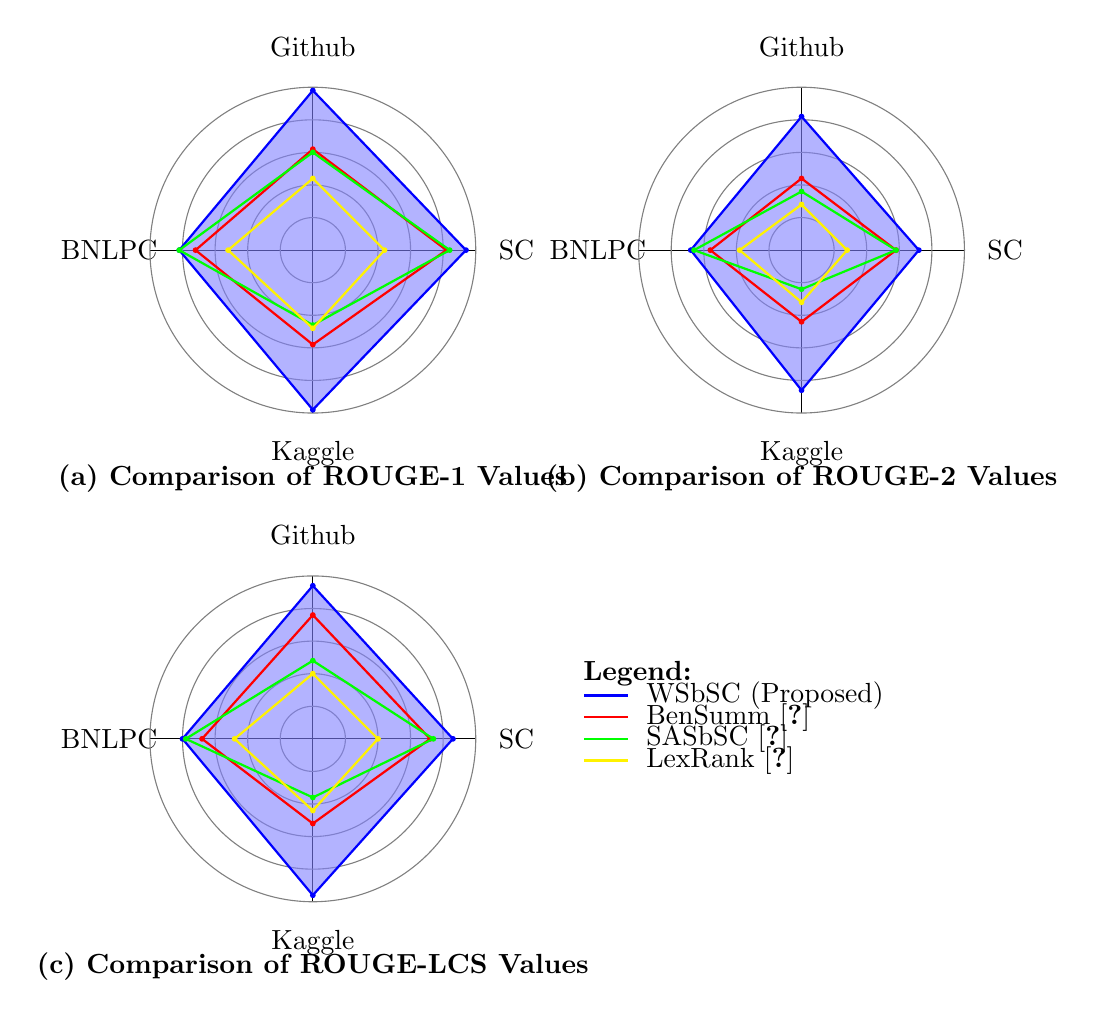
\begin{tikzpicture}[scale=0.002*\textwidth]
    % Define the number of axes (dimensions)
    \def\n{4}
    % Define the names of the features
    \def\features{{"SC", "Kaggle", "BNLPC", "Github"}}
    % Define the maximum value
    \def\maxvalue{5}

    % Define values for three different radar charts
    \def\valuesAW{{4.7, 4.9, 4.1, 4.9}}
    \def\valuesAB{{4.1, 2.9, 3.6, 3.1}}
    \def\valuesAS{{4.2, 2.3, 4.1, 3.0}}
    \def\valuesAL{{2.2, 2.4, 2.6, 2.2}}

    \def\valuesBW{{3.6, 4.3, 3.4, 4.1}}
    \def\valuesBB{{2.9, 2.2, 2.8, 2.2}}
    \def\valuesBS{{2.9, 1.2, 3.3, 1.8}}
    \def\valuesBL{{1.4, 1.6, 1.9, 1.4}}

    \def\valuesCW{{4.3, 4.8, 4.0, 4.7}}
    \def\valuesCB{{3.6, 2.6, 3.4, 3.8}}
    \def\valuesCS{{3.7, 1.8, 3.9, 2.4}}
    \def\valuesCL{{2.0, 2.2, 2.4, 2.0}}

    % First Radar Chart (Top-left quarter)
    \begin{scope}[xshift=-5cm, yshift=5cm, scale=0.6]
        %write the dataset labels
        \foreach \i in {1,...,\n} {
            \draw (90-\i*360/\n:5) -- (0,0);
            \node at (90-\i*360/\n:6.25) {\pgfmathparse{\features[\i-1]}\pgfmathresult};
        }
        %draw the circle
        \node at (90-2*360/4:7){\textbf{(a) Comparison of ROUGE-1 Values}};
        \foreach \j in {1,...,\maxvalue} {
            \draw[gray, thin] (0,0) circle (\j);
        }

        %draw wsbsc
        \foreach \i [evaluate={\angle=90-\i*360/\n; \valueAW=\valuesAW[\i-1];}] in {1,...,\n} {
            \coordinate (PA\i) at (\angle:\valueAW);
            \filldraw[blue] (PA\i) circle (2pt);
        }
        \fill[blue!50, opacity=0.6] (PA1) -- (PA2) -- (PA3) -- (PA4) -- cycle;
        \foreach \i in {1,...,\n} {
            \pgfmathtruncatemacro{\nexti}{mod(\i,\n)+1}
%                    \draw [thick, cyan] plot [smooth, tension=2] coordinates { (PA\i) (PA\nexti)};
            \draw[thick, blue] (PA\i) -- (PA\nexti);
        }
%                \draw [thick,cyan] plot [smooth cycle, tension=1] coordinates { (PA1) (PA2) (PA3) (PA4)};

        %draw bensumm
        \foreach \i [evaluate={\angle=90-\i*360/\n; \valueAB=\valuesAB[\i-1];}] in {1,...,\n} {
            \coordinate (PB\i) at (\angle:\valueAB);
            \filldraw[red] (PB\i) circle (2pt);
        }
        \foreach \i in {1,...,\n} {
            \pgfmathtruncatemacro{\nexti}{mod(\i,\n)+1}
            \draw[thick, red] (PB\i) -- (PB\nexti);
        }

%                draw sasbsc
        \foreach \i [evaluate={\angle=90-\i*360/\n; \valueAS=\valuesAS[\i-1];}] in {1,...,\n} {
            \coordinate (PC\i) at (\angle:\valueAS);
            \filldraw[green] (PC\i) circle (2pt);
        }
        \foreach \i in {1,...,\n} {
            \pgfmathtruncatemacro{\nexti}{mod(\i,\n)+1}
            \draw[thick, green] (PC\i) -- (PC\nexti);
        }

        %draw lexrank
        \foreach \i [evaluate={\angle=90-\i*360/\n; \valueAL=\valuesAL[\i-1];}] in {1,...,\n} {
            \coordinate (PD\i) at (\angle:\valueAL);
            \filldraw[yellow] (PD\i) circle (2pt);
        }
        \foreach \i in {1,...,\n} {
            \pgfmathtruncatemacro{\nexti}{mod(\i,\n)+1}
            \draw[thick, yellow] (PD\i) -- (PD\nexti);
        }
    \end{scope}

    % Second Radar Chart (Top-right quarter)
    \begin{scope}[xshift=4cm, yshift=5cm, scale=0.6]
        \foreach \i in {1,...,\n} {
            \draw (90-\i*360/\n:5) -- (0,0);
            \node at (90-\i*360/\n:6.25) {\pgfmathparse{\features[\i-1]}\pgfmathresult};
        }
        \node at (90-2*360/4:7){\textbf{(b) Comparison of ROUGE-2 Values}};
        \foreach \j in {1,...,\maxvalue} {
            \draw[gray, thin] (0,0) circle (\j);
        }

        \foreach \i [evaluate={\angle=90-\i*360/\n; \valueBW=\valuesBW[\i-1];}] in {1,...,\n} {
            \coordinate (PA\i) at (\angle:\valueBW);
            \filldraw[blue] (PA\i) circle (2pt);
        }
        \fill[blue!50, opacity=0.6] (PA1) -- (PA2) -- (PA3) -- (PA4) -- cycle;
        \foreach \i in {1,...,\n} {
            \pgfmathtruncatemacro{\nexti}{mod(\i,\n)+1}
            \draw[thick, blue] (PA\i) -- (PA\nexti);
        }

        \foreach \i [evaluate={\angle=90-\i*360/\n; \valueBB=\valuesBB[\i-1];}] in {1,...,\n} {
            \coordinate (PB\i) at (\angle:\valueBB);
            \filldraw[red] (PB\i) circle (2pt);
        }
        \foreach \i in {1,...,\n} {
            \pgfmathtruncatemacro{\nexti}{mod(\i,\n)+1}
            \draw[thick, red] (PB\i) -- (PB\nexti);
        }

        \foreach \i [evaluate={\angle=90-\i*360/\n; \valueBS=\valuesBS[\i-1];}] in {1,...,\n} {
            \coordinate (PC\i) at (\angle:\valueBS);
            \filldraw[green] (PC\i) circle (2pt);
        }
        \foreach \i in {1,...,\n} {
            \pgfmathtruncatemacro{\nexti}{mod(\i,\n)+1}
            \draw[thick, green] (PC\i) -- (PC\nexti);
        }

        \foreach \i [evaluate={\angle=90-\i*360/\n; \valueBL=\valuesBL[\i-1];}] in {1,...,\n} {
            \coordinate (PD\i) at (\angle:\valueBL);
            \filldraw[yellow] (PD\i) circle (2pt);
        }
        \foreach \i in {1,...,\n} {
            \pgfmathtruncatemacro{\nexti}{mod(\i,\n)+1}
            \draw[thick, yellow] (PD\i) -- (PD\nexti);
        }
    \end{scope}

    % Third Radar Chart (Bottom-left quarter)
    \begin{scope}[xshift=-5cm, yshift=-4cm, scale=0.6]
        \foreach \i in {1,...,\n} {
            \draw (90-\i*360/\n:5) -- (0,0);
            \node at (90-\i*360/\n:6.25) {\pgfmathparse{\features[\i-1]}\pgfmathresult};
        }
        \node at (90-2*360/4:7){\textbf{(c) Comparison of ROUGE-LCS Values}};
        \foreach \j in {1,...,\maxvalue} {
            \draw[gray, thin] (0,0) circle (\j);
        }

        \foreach \i [evaluate={\angle=90-\i*360/\n; \valueCW=\valuesCW[\i-1];}] in {1,...,\n} {
            \coordinate (PA\i) at (\angle:\valueCW);
            \filldraw[blue] (PA\i) circle (2pt);
        }
        \fill[blue!50, opacity=0.6] (PA1) -- (PA2) -- (PA3) -- (PA4) -- cycle;
        \foreach \i in {1,...,\n} {
            \pgfmathtruncatemacro{\nexti}{mod(\i,\n)+1}
            \draw[thick, blue] (PA\i) -- (PA\nexti);
        }

        \foreach \i [evaluate={\angle=90-\i*360/\n; \valueCB=\valuesCB[\i-1];}] in {1,...,\n} {
            \coordinate (PB\i) at (\angle:\valueCB);
            \filldraw[red] (PB\i) circle (2pt);
        }
        \foreach \i in {1,...,\n} {
            \pgfmathtruncatemacro{\nexti}{mod(\i,\n)+1}
            \draw[thick, red] (PB\i) -- (PB\nexti);
        }

        \foreach \i [evaluate={\angle=90-\i*360/\n; \valueCS=\valuesCS[\i-1];}] in {1,...,\n} {
            \coordinate (PC\i) at (\angle:\valueCS);
            \filldraw[green] (PC\i) circle (2pt);
        }
        \foreach \i in {1,...,\n} {
            \pgfmathtruncatemacro{\nexti}{mod(\i,\n)+1}
            \draw[thick, green] (PC\i) -- (PC\nexti);
        }

        \foreach \i [evaluate={\angle=90-\i*360/\n; \valueCL=\valuesCL[\i-1];}] in {1,...,\n} {
            \coordinate (PD\i) at (\angle:\valueCL);
            \filldraw[yellow] (PD\i) circle (2pt);
        }
        \foreach \i in {1,...,\n} {
            \pgfmathtruncatemacro{\nexti}{mod(\i,\n)+1}
            \draw[thick, yellow] (PD\i) -- (PD\nexti);
        }
    \end{scope}

    % Legend (Bottom-right quarter)
    \begin{scope}[xshift=4cm, yshift=-4cm, scale=0.8]
        \node[anchor=west] at (-5.25, 1.5) {\textbf{Legend:}};
        \draw[thick, blue] (-5, 1) -- (-4, 1);
        \node[anchor=west] at (-3.8, 1) {WSbSC (Proposed)};

        \draw[thick, red] (-5, 0.5) -- (-4, 0.5);
        \node[anchor=west] at (-3.8, 0.5) {BenSumm~\cite{chowdhury-etal-2021-tfidf-clustering}};

        \draw[thick, green] (-5, 0) -- (-4, 0);
        \node[anchor=west] at (-3.8, 0) {SASbSC~\cite{roychowdhury-etal-2022-spectral-base}};

        \draw[thick, yellow] (-5, -0.5) -- (-4, -0.5);
        \node[anchor=west] at (-3.8, -0.5) {LexRank~\cite{Erkan-lexRank-2004}};
    \end{scope}
\end{tikzpicture}